%% ============================================================
%% IST (Information and Software Technology) manuscript
%% Why Is It So Hard to Localize Bugs in Model Context Protocol (MCP) Pipelines?
%% An Empirical Study with a Reproducible Fault-Injection Benchmark
%% Authors: Kehui Chen, Yicheng Sun, Jacky Keung, Zhenyu Mao, Xiaoxue Ma
%% Template: Elsevier CAS (cas-dc).
%% Each section is \input from its own file (sec_*.tex) for easy editing.
%% ============================================================

\documentclass[a4paper,fleqn]{cas-dc}

%\documentclass[a4paper,fleqn,longmktitle]{cas-dc}

\usepackage[authoryear,longnamesfirst]{natbib}
\usepackage{algorithmic}
\usepackage{algorithm}
\usepackage{multirow}
\usepackage{multicol}
\usepackage{makecell}
\usepackage{graphicx}
\usepackage{textcomp}
\usepackage{xcolor}
\usepackage{booktabs} % professional table rules used in main_body.tex
\usepackage{microtype} % improves line breaking and reduces overfull boxes
\usepackage{xurl} % allows robust line breaks in long URLs/identifiers
\usepackage{tabularx}
\usepackage{array}
\usepackage{ragged2e}
\usepackage{placeins}
\usepackage{caption}
\usepackage{fontawesome5}

% Compact, publication-style float spacing for a two-column Elsevier layout.
\setlength{\textfloatsep}{10pt plus 2pt minus 2pt}
\setlength{\floatsep}{9pt plus 2pt minus 2pt}
\setlength{\intextsep}{9pt plus 2pt minus 2pt}
\setlength{\dbltextfloatsep}{10pt plus 2pt minus 2pt}
\setlength{\dblfloatsep}{9pt plus 2pt minus 2pt}


\def\tsc#1{\csdef{#1}{\textsc{\lowercase{#1}}\xspace}}
\tsc{WGM}
\tsc{QE}

\begin{document}
\let\WriteBookmarks\relax
\def\floatpagepagefraction{1}
\def\textpagefraction{.001}
\let\printorcid\relax

% Short title
\shorttitle{Why MCP Fault Localization Is Hard}

% Short author
\shortauthors{K. Chen et al.}

% Main title of the paper
\title [mode = title]{Why Is It So Hard to Localize Bugs in Model Context Protocol (MCP)
Pipelines? An Empirical Study with a Reproducible Fault-Injection Benchmark}

% Title footnote
\tnotemark[1]
\tnotetext[1]{This work is partially supported by the Research Grants Council (RGC) of the
Hong Kong Special Administrative Region, China under the General Research Fund
(UGC/FDS16/E27/25), Hong Kong Metropolitan University Research Grant (RD/2025/1.24), and
research funds from City University of Hong Kong (6000871, 9229109, 9229192).}

% First author
\author[1]{Kehui Chen}
\ead{kehuichen2-c@my.cityu.edu.hk}

% \author[1]{Yicheng Sun}
% \ead{yicsun2-c@my.cityu.edu.hk}

\author[1]{Jacky Keung}
\ead{Jacky.Keung@cityu.edu.hk}

% \author[1]{Zhenyu Mao}
% \ead{zhenyumao2-c@my.cityu.edu.hk}

\author[2]{Xiaoxue Ma\cormark[1]}
\ead{kxma@hkmu.edu.hk}
\cortext[cor1]{Corresponding author}

\affiliation[1]{organization={Department of Computer Science, City University of Hong Kong},
            city={Kowloon},
            country={Hong Kong SAR}}

\affiliation[2]{organization={Department of Computer Science, Hong Kong Metropolitan University},
            city={Kowloon},
            country={Hong Kong SAR}}

% Abstract (structured: Context / Objective / Methods / Results / Conclusion)
\begin{abstract}
\noindent \textbf{Context}: Large language models (LLMs) are increasingly used in AI-driven
software engineering through the Model Context Protocol (MCP), which orchestrates external
tools across the Host, Client, and Server components and the transport between them. Yet
practitioners report that localizing the root cause of a runtime fault is extremely difficult.

\noindent \textbf{Objective}: This study investigates \emph{why} MCP fault localization is so
hard, and whether automated diagnostic guidance can alleviate it. It aims to move beyond
subjective industrial complaints to objective, reproducible technical evidence.

\noindent \textbf{Methods}: We adopt a sequential-exploratory mixed-methods design. First, we
conduct semi-structured interviews with 20 MCP practitioners from FinTech and Internet
enterprises, and analyse the data with open coding. Second, guided by the reported
fault-diagnosis pain points, we define a four-layer runtime fault taxonomy and build a
\textbf{real-bug dataset} by mining the entire issue tracker of the official
\verb|modelcontextprotocol/python-sdk|: a funnel of 1,343 pure issues to 398
confirmed real bugs to 342 active (56 already fixed in the
pinned SDK removed), of which \textbf{49 are reproduced at runtime} over the production
Streamable-HTTP transport, each bound to a real issue number. We then run a genuine LLM
diagnosis over these 49 bugs and compare its localisation accuracy with and without the output
of a runnable diagnostic-clue tool that classifies the exposure channel and emits directional
guidance without revealing the root-cause layer.

\noindent \textbf{Results}: Interviews identify fault localization as the leading operational
obstacle. Controlled experiments over the 49 reproduced real bugs derive a \emph{three-channel
exposure model}: non-Server MCP faults are pushed to the Server layer (7/13), silently
swallowed (3/13 non-Server, 11/49 = 22.4\% overall), or surfaced as raw Python exceptions in
the calling code (3/13); a further 17/49 = 34.7\% of Server-origin bugs are \emph{genericised},
their real root cause replaced by a generic message. A genuine LLM reading only the SDK's
reported error text achieves 77.6\% overall but only \textbf{15.4\%} on the 13 non-Server bugs
(0\% on both Host- and Client-origin faults, which are all pushed onto the Server, and only
23.1\% at Top-1); a runnable diagnostic-clue tool that packages the exposure channel into
directional guidance --- without revealing the origin layer --- raises non-Server accuracy to
23.1\% (+7.7 pp), whereas a bare channel-label control does not help (0\%).

\noindent \textbf{Conclusion}: MCP fault localization is hard primarily because default SDK
error reporting routes faults through distinct channels that hide the true origin, and
lacks root-cause layer metadata. Honest, automated diagnostic guidance that packages these
channels measurably improves localization of the hard non-Server faults. A repair experiment
confirms the difficulty is localization rather than fixing: given the full source an LLM
repairs 69.6\% of the auto-verifiable cases with or without the guidance. We release the
real-bug dataset to support future research on MCP reliability and fault diagnosis.
\end{abstract}

% Keywords
\begin{keywords}
Model Context Protocol \sep
Fault localization \sep
Root-cause analysis \sep
Large language models \sep
Observability \sep
Empirical software engineering
\end{keywords}

\maketitle

% Main content (each part in its own file for easy editing)
% ============================================================
% 正文：Introduction
% 作者：Kehui Chen, Jacky Keung, Xiaoxue Ma
% 主题：MCP 故障定位（fault localization）根因实证研究
% ============================================================

\section{Introduction}\label{sec:intro}

\noindent Large language models (LLMs) are increasingly deployed in enterprise software
engineering, yet they struggle with cross-system invocation and multi-tool collaboration
\cite{hou2025model}\cite{yang2025survey}. To tackle this, Anthropic released the Model
Context Protocol (MCP) in late 2024 \cite{anthropic_mcp_2024}. MCP acts as a middle-layer
protocol that connects LLMs to external resources through four core components: Host,
Client, Server, and Resource \cite{yang2025survey}. It standardises tool invocation and
context exchange across heterogeneous systems, and has become a foundation for many
LLM-driven workflows in industry.

Existing MCP research largely falls into three directions: benchmark construction for
real-world LLM evaluation \cite{liu2025mcpeval}\cite{yang2025mcpsecbench}, system
integration and performance optimisation \cite{xu2025towards}\cite{li2025energyplus}, and
security-threat analysis with countermeasures \cite{hasan2025model}\cite{mcpSecurity2025}.
Most benchmarks focus on adversarial security attacks or high-level functional evaluation,
while comparatively little attention has been paid to \emph{ordinary runtime faults} and
the \emph{observability issues} that arise in real-world MCP deployments.

Despite these technical advances, empirical evidence on how MCP behaves in production
remains scarce. In particular, practitioners consistently report that \emph{it is
extremely difficult to localise the root cause of a fault} in an MCP pipeline. The
difficulty is not merely a subjective complaint: it stems from the way MCP SDKs report
errors. A single call runs between the Host, Client, and Server components, and a fault may
arise in any of them or during the transport of the messages between them; yet the layer at
which the resulting error is \emph{displayed} often differs from the component in which the
fault actually \emph{originated}. Moreover, some erroneous inputs are silently accepted by
the SDK and return a successful status without any error flag, making these defects
invisible to ordinary monitoring pipelines.

Existing empirical evidence on MCP adoption originates mostly from practitioner
interviews \cite{ma2025practitioners} or open-source issue mining. While interviews capture
subjective industrial pain points, they cannot provide \emph{controlled, reproducible}
technical evidence that explains \emph{why} certain problems occur. To our best knowledge,
there is still no end-to-end, runnable fault dataset for MCP runtime failure analysis. This
creates a gap between perceived real-world difficulties and verifiable technical root
causes.

To narrow this gap, we adopt a \emph{sequential-exploratory mixed-methods} research design.
In the first phase, we obtain direct insights from enterprise practitioners through
semi-structured interviews to identify the core pain points of MCP deployment, with special
attention to fault diagnosis. In the second phase, guided by these pain points, we mine a
\textbf{real-bug dataset} --- a complete census of the official
\verb|modelcontextprotocol/python-sdk| issue tracker (from 1,343 pure issues to 398
confirmed real bugs to 342 active after removing the 56 already
fixed in the pinned SDK), reproduce \textbf{49} of them at runtime over the production
Streamable-HTTP transport, and run observability experiments that empirically examine the
technical roots of fault-localisation difficulty. This triangulation connects qualitative
practitioner insight with objective experimental observation, and lets us quantify why fault
localisation in MCP is so hard.

Concretely, this work addresses the following research questions:
\begin{itemize}
  \item \textbf{RQ1} What types of runtime faults can occur across the four-layer MCP
        fault taxonomy (Host, Client, Server, Transport)?
  \item \textbf{RQ2} To what extent does MCP SDK error reporting suffer from
        \emph{manifestation-root-cause mismatch}, i.e.\ errors surfaced at one layer while
        the true root cause lies in another?
  \item \textbf{RQ3} To what extent does MCP SDK error reporting exhibit \emph{silent
        failures}, i.e.\ erroneous inputs that return a successful status without an error
        flag?
  \item \textbf{RQ4} What are the technical root causes that make MCP fault localisation
        difficult, and how can automated diagnostic guidance alleviate them?
\end{itemize}

The main contributions of this paper are summarised as follows:
\begin{enumerate}
  \item We present interview evidence of MCP adoption from 20 real-world practitioners
        across Internet and FinTech enterprises, characterising fault-diagnosis as the
        leading operational obstacle (Section~\ref{sec:results}).
  \item We define a four-layer MCP runtime-fault taxonomy (Host scheduling, Client message,
        Server tool, Transport) and build a \textbf{real-bug dataset} by mining the entire
        issue tracker of the official \verb|modelcontextprotocol/python-sdk|, reproducing
        \textbf{49} genuine bugs at runtime over the production Streamable-HTTP transport
        (Sections~\ref{sec:method},~\ref{sec:setup}).
  \item We empirically derive a \emph{three-channel exposure model} characterising how MCP
        faults actually surface: \emph{pushed-to-Server} (7/13 non-Server bugs),
        \emph{silent failure} (11/49 = 22.4\%), and \emph{caller-exception} (3/13); a further
        17/49 = 34.7\% are \emph{genericised}, their real root cause replaced by a generic
        message. None of the 13 non-Server bugs is localised at its true origin (10/13 = 76.9\%
        generalised mismatch).
  \item We build a genuine LLM diagnosis baseline: a model (DeepSeek-V4 via a CityU OpenAI
        proxy) that reads only the true SDK error text and predicts the root-cause layer
        achieves 77.6\% overall but only \textbf{15.4\%} on the 13 non-Server bugs (0\% on both
        Host- and Client-origin faults, misattributed to the Server layer), and the non-Server
        Top-K is only 23.1\% at Top-1 (84.6\% at Top-3).
  \item We design a \emph{runnable diagnostic-clue tool} that classifies the exposure channel
        and emits directional guidance without revealing the root-cause layer, and show it
        raises the non-Server localisation accuracy from 15.4\% to 23.1\% (+7.7 pp), whereas a
        bare channel-label control does not help (0\%), evidencing the value of honest,
        non-leaking diagnostic guidance.
  \item We run a repair experiment and find the clue \emph{does not} change repair success
        (69.6\% with or without it on the auto-verifiable subset), because with the full source
        the LLM reads the fault directly --- corroborating that localisation, not code-fixing,
        is the bottleneck in MCP debugging.
  \item We release the fault dataset, source scripts, and raw execution records, and derive
        actionable observability recommendations for future MCP protocol and SDK design.
\end{enumerate}

The remainder of this paper is organised as follows.
Section~\ref{sec:related} reviews related work on LLM tool integration, MCP background, and
existing fault-taxonomy research.
Section~\ref{sec:method} describes our mixed-methods methodology and defines the four-layer
fault taxonomy.
Section~\ref{sec:setup} details the real-bug dataset construction, the four-layer taxonomy
and the controlled reproduction / observability experiment configuration.
Section~\ref{sec:results} reports both the demand-side interview evidence and the results
of the fault-injection and diagnosis experiments.
Section~\ref{sec:discussion} discusses research and practical implications, together with
threats to validity.
Finally, Section~\ref{sec:concl} concludes the paper.
% ============================================================
% 正文：Related Work and Background
% 作者：Kehui Chen, Jacky Keung, Xiaoxue Ma
% 主题：MCP 故障定位（fault localization）根因实证研究
% ============================================================

\section{Related Work and Background}\label{sec:related}

This section reviews the evolution of LLM tool integration, core MCP concepts, existing
fault-taxonomy research, and the gaps our work addresses.

\subsection{Evolution of LLM Tool Integration}

LLM-external tool integration has evolved through three phases to improve collaboration and
ecosystem compatibility \cite{liu2024toolace}.

\textbf{Early single-tool function calling.} Proposed by OpenAI's function-calling API, this
phase supports isolated tool invocations such as calculators and search engines
\cite{zhang2024large}. It cannot preserve cross-tool context, so task metadata must be
retransmitted for each call, making complex multi-step workflows unsupported
\cite{kim2024llm}\cite{wang2025function}.

\textbf{Second-stage agent orchestration frameworks.} Frameworks such as LangChain and
AutoGPT support chained tool calls through task planning and selection \cite{lin2025mao}.
Their proprietary protocols form isolated ecosystems and raise migration costs
\cite{haddad2017connecting}.

\textbf{Current-stage standardised middleware protocols.} As a standardised middleware, MCP
uses unified interfaces to break platform barriers \cite{anthropic_mcp_2024}\cite{hou2025model}.
It avoids vendor lock-in and enables cross-system collaboration for large-scale enterprise
deployment.

\subsection{The Model Context Protocol}

MCP is a standard middleware for LLM-tool collaboration. It resolves context fragmentation,
inconsistent interaction, and tight coupling to realise efficient, secure cross-system
cooperation. It consists of four core components (Host, Client, Server, and Resource
\cite{yang2025survey}), whose main features are:

\textbf{Unified context abstraction.} MCP adopts standard task-context formats for user
preferences, logs, and security policies, ensuring consistent data transmission and parsing.

\textbf{Decoupled layered architecture.} MCP decouples the LLM and tool layers so that each
can evolve independently, improving scalability and maintainability.

\textbf{Distributed dynamic context management.} MCP supports real-time context update,
sharing, and fine-grained access control to guarantee context security and consistency in
distributed systems.

\subsection{Current Research on MCP}

\textbf{MCP benchmarks.} A series of MCP benchmarks has been proposed for real-world LLM
evaluation, overcoming defects of early testing systems \cite{liu2025mcpeval}\cite{yang2025mcpsecbench}.

\textbf{MCP integration and performance.} Studies explore embedding MCP into existing systems
for performance improvement \cite{xu2025towards}\cite{li2025energyplus}\cite{da2025beyond}.

\textbf{Security and compliance.} MCP security is widely studied; researchers have classified
attacks and built defense frameworks \cite{hasan2025model}. Seventeen attack types and basic
protections such as access control and audit logging have been presented
\cite{yang2025mcpsecbench}\cite{mcpSecurity2025}\cite{fu2025mcp}. Most defenses remain passive.

\subsection{Fault Taxonomies and Fault-Oriented Benchmarks}

Recent work has begun to analyse failure modes in MCP deployments. Existing fault taxonomies
are mostly derived by mining GitHub issue reports and open-source repository discussions,
and identify several failure categories predominantly observed on the MCP Server side.
Security-oriented benchmarks such as MCPSecBench mainly construct adversarial attack
scenarios for vulnerability testing \cite{yang2025mcpsecbench}.

Nevertheless, existing fault-related work has three limitations. First, analyses based on
issue mining rely on static text reports rather than executable, end-to-end test cases, so
faults cannot be directly reproduced in controlled experiments. Second, existing taxonomies
place heavy emphasis on Server-side and security-oriented failures, giving limited attention
to faults originating from Host, Client, or Transport layers; ordinary operational runtime
faults and SDK observability behaviours remain underexplored. Third, existing studies
rarely investigate error-reporting phenomena such as manifestation-root-cause mismatch or
silent failure, which strongly affect the real-world debugging experience.

\subsubsection{Why a New Four-Layer Taxonomy? (Comparison with Existing Fault Taxonomies)}

To situate our work in the broader software-engineering literature, we build on the large-scale
empirical taxonomy of MCP faults recently proposed by Taraghi and co-workers
\cite{taraghi2026real}, who mined 3,282 bug-related GitHub issues and derived five high-level
fault categories (e.g.\ \texttt{Server/Tool Configuration} 31.74\%, \texttt{Server/Host
Configuration} 28.64\%, \texttt{Server Setting} 27.45\%), validated by a survey of 41
practitioners. Applied to our dataset, MCP faults would fall into a small number of these
categories: \emph{configuration-related} failures (triggered by erroneous
tool/parameter/credential configuration, e.g.\ \texttt{Server/Host Configuration},
\texttt{Server/Tool Configuration}) and \emph{general programming} failures (triggered by a
bug inside the tool's own execution logic, e.g.\ \texttt{General Programming}). Each reproduced
real bug in our dataset is mapped to such a category in Section~\ref{sec:setup}.

Crucially, Taraghi et al.\ identify \emph{diagnostic friction} as a key issue (their Findings
F4/F5 and insight A4) and recommend making host-side and protocol-boundary failures
\emph{observable}. However, their study is issue- and survey-based: it \emph{describes} which MCP
faults are hard to diagnose, but provides no controlled, reproducible mechanism to measure
\emph{why} diagnosis fails for specific fault types. Comparing their taxonomy with our four-layer
scheme highlights the gap we address. Taraghi's taxonomy classifies a fault by its \emph{trigger
type} and architectural \emph{boundary of resolution}, but it does not distinguish \emph{where
the fault originates} from \emph{where the fault is reported}. In an MCP pipeline, a single tool
call runs between the Host, Client, and Server components, and a fault may arise in any of them
or during transport between them; yet the SDK exposes the resulting error at only one layer.
Consequently, many MCP faults are triggered by a configuration or
programming error at one layer, but are \emph{reported} at the Server layer. The Taraghi
categories therefore describe the \emph{nature} of the defect but cannot express its
\emph{location}, which is exactly the information a developer needs when localising a fault.

Our four-layer taxonomy addresses this gap by classifying each fault by the architectural layer
at which it \emph{originates} (Host scheduling, Client message, Server tool, or Transport). This
makes two properties explicit that prior taxonomies obscure: (i) the \emph{cross-component}
nature of MCP faults, in which the reported layer differs from the originating layer, and (ii)
the \emph{manifestation-root-cause separation} that makes localisation uniquely difficult. The
two taxonomies are therefore \emph{complementary} rather than competing: Taraghi explains
\emph{what kind of bug} occurs and \emph{where it is resolved}, whereas our taxonomy explains
\emph{where it originates and how it is (mis)reported}. Moreover, whereas Taraghi stops at
recommending observability, our benchmark \emph{measures} it: we quantify the three channels
through which faults evade localisation and show that a runnable diagnostic-clue tool improves
it. We adopt the latter as our primary dimension because it directly supports fault
localisation and observability.

\subsection{Research Gaps and Motivation}

Existing MCP studies have clear limitations for enterprise deployment. First, most
benchmarks are laboratory-based and lack real enterprise data \cite{liu2025mcpeval}.
Second, integration research concentrates on technical embedding, ignoring practical
deployment challenges \cite{xu2025towards}\cite{li2025energyplus}. Third, security studies
focus on attack discovery and passive defence \cite{hasan2025model}. Fourth, empirical
studies relying purely on interviews or issue mining deliver subjective observations without
reproducible technical evidence to verify \emph{why} deployment pain points occur. Fifth,
there is a shortage of executable end-to-end fault datasets targeting general MCP runtime
failures, which hinders controlled experimental research on fault diagnosis and
observability.
% ============================================================
% 正文：Research Methodology
% 作者：Kehui Chen, Jacky Keung, Xiaoxue Ma
% 主题：MCP 故障定位（fault localization）根因实证研究
% ============================================================

\section{Research Methodology}\label{sec:method}

We adopt a sequential-exploratory mixed-methods design combining qualitative and
quantitative evidence \cite{ostlund2011combining}. The overview is shown in Fig.~\ref{fig:methodology}.

The design has two phases. \textbf{Phase 1 (demand side):} semi-structured interviews with
MCP practitioners capture the perceived pain points of MCP adoption, with particular focus
on fault diagnosis. \textbf{Phase 2 (technical side):} guided by these pain points, we mine a
real-bug dataset from the official MCP SDK issue tracker, reproduce a subset at runtime, and
run observability experiments to quantify the technical root causes. The two phases are
triangulated: interview findings motivate the experimental design, and experimental results
objectively verify the interview complaints.

\noindent
\begin{minipage}{\linewidth}
  \centering
  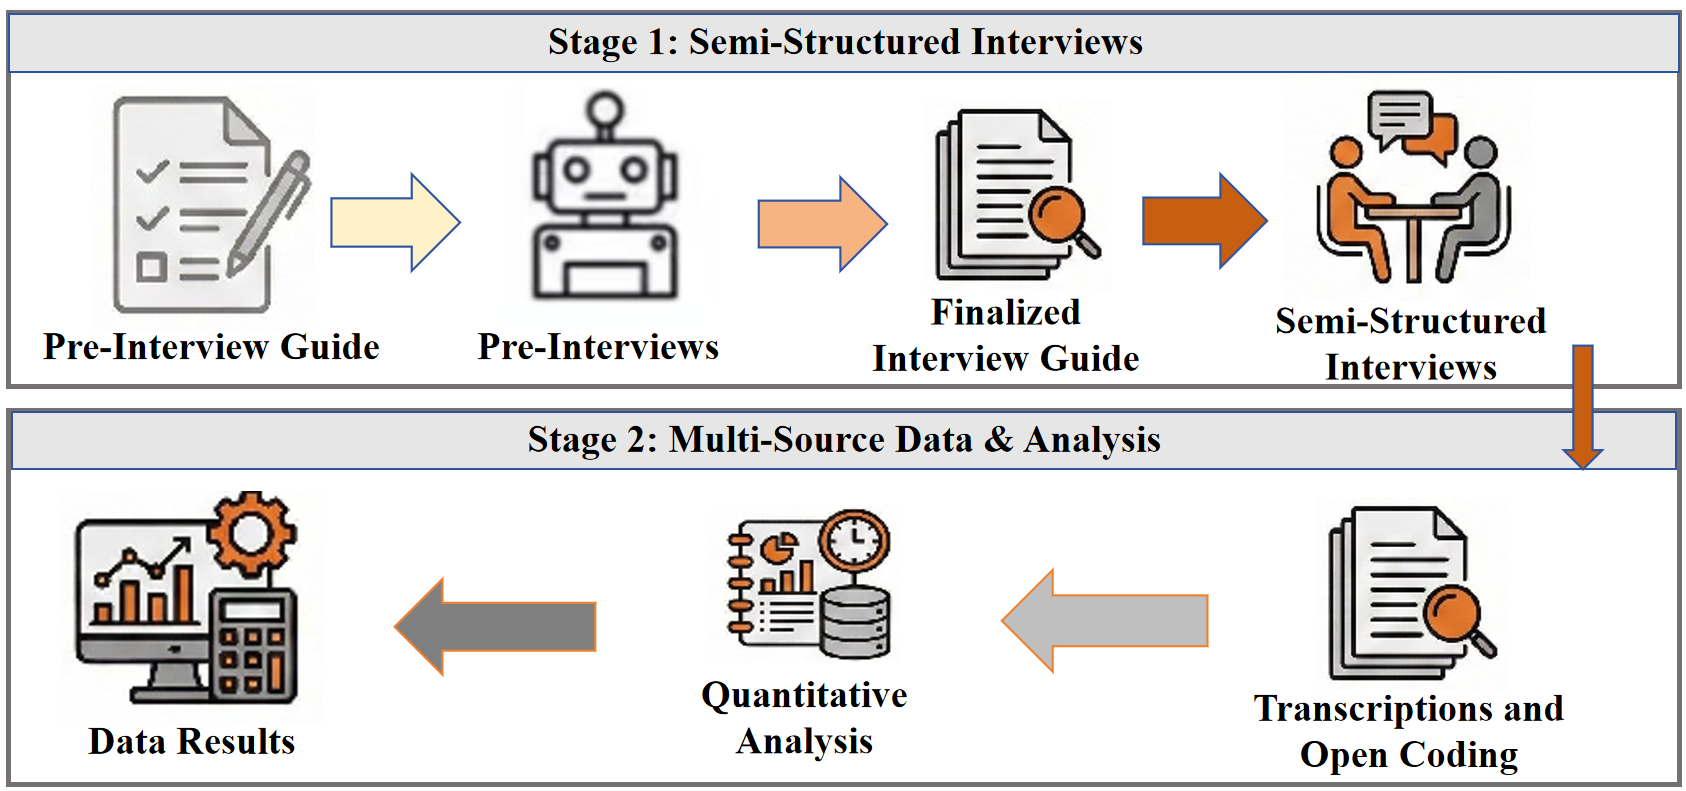
\includegraphics[width=\linewidth]{figs/methodology}
  \captionof{figure}{Overview of the sequential-exploratory mixed-methods methodology.}
  \label{fig:methodology}
\end{minipage}

\subsection{Phase 1: Semi-Structured Interviews}

We use expert sampling, a subtype of purposive sampling \cite{baltes2022sampling}, and
conduct semi-structured interviews with 20 practitioners in the MCP field, preceded by three
pre-interviews to refine the interview guide \cite{adeoye2021research}.

\textbf{Interview design.} We drafted initial questions from the literature
\cite{ma2025practitioners} and revised them through pre-interviews. The final guide contains
open-ended questions \cite{le2014loaded}; participants could answer ``I don't know'' to reduce
response bias. We finalised 31 core questions covering demographics, MCP practices and
problems, technical capability assessment, security and privacy, future expectations, and
counterintuitive insights.

\textbf{Procedure.} We conducted pre-interviews with three participants; formal interviews
were held online, each lasting 90--120 minutes, and were transcribed verbatim (~400,000 words
of original data). We conducted secondary interviews with ten key participants (30 minutes
each) to clarify vague views. Sample size was determined by theoretical saturation: no new
viewpoints appeared after 20 interviews \cite{ma2025practitioners}.

\textbf{Participants.} We recruited 20 MCP practitioners from FinTech and Internet industries
(e.g., HSBC, Huawei); 9 from FinTech and 11 from Internet. Participants cover all core MCP
roles (Host, Client, Server, User) and multiple job roles (Senior Architect, Software
Developer, Business Analyst, Algorithm Designer), as summarised in
Table~\ref{tab:participants}. Experience ranges from 2 to 20 years; team sizes range from 6
to 160 people.

\begin{table}[!t]
\centering
\caption{Participant demographics and experience distribution.}
\label{tab:participants}
\scriptsize
\renewcommand{\arraystretch}{1.05}
\setlength{\tabcolsep}{1.6pt}
\begin{tabular}{@{}c c c c c c c@{}}
\toprule
\textbf{ID} & \textbf{Role} & \textbf{Ind.} & \textbf{MCP} & \textbf{Mgmt.} & \textbf{Exp.} & \textbf{Team} \\
\midrule
P1  & SA & F & H/C/S & Y & $>$10 & $>$80 \\
P2  & SA & I & H/C/S & Y & $>$10 & $>$80 \\
P3  & SA & I & H/C/S & Y & $>$10 & $>$80 \\
P4  & SA & I & H/C/S & Y & 3--10 & 21--40 \\
P5  & SD & F & C/S   & N & 3--10 & 21--40 \\
P6  & SD & I & C/S   & N & 3--10 & 21--40 \\
P7  & SD & F & C/S   & N & 3--10 & 21--40 \\
P8  & SD & I & C/S   & N & 3--10 & 21--40 \\
P9  & SD & F & C/S   & N & 3--10 & 21--40 \\
P10 & SD & I & C/S   & N & 3--10 & 21--40 \\
P11 & SD & F & C/S   & N & 3--10 & 41--80 \\
P12 & SD & I & C/S   & N & 3--10 & 41--80 \\
P13 & SD & F & S     & N & 3--10 & 41--80 \\
P14 & SD & I & S     & N & $<$3 & 41--80 \\
P15 & BA & F & U     & N & 3--10 & 21--40 \\
P16 & BA & I & U     & N & 3--10 & 21--40 \\
P17 & BA & F & U     & N & 3--10 & 21--40 \\
P18 & BA & I & U     & N & 3--10 & 41--80 \\
P19 & AD & F & S     & Y & 3--10 & 21--40 \\
P20 & AD & I & S     & Y & $>$10 & $>$80 \\
\bottomrule
\end{tabular}
\vspace{0.35em}
\parbox{\columnwidth}{\scriptsize\raggedright
\textit{Note:} SA = Senior Architect; SD = Software Developer; BA = Business Analyst; AD = Algorithm Designer; F = FinTech; I = Internet; H/C/S = Host/Client/Server; C/S = Client/Server; S = Server; U = User; Y/N = management responsibility. Experience is reported in years.}
\end{table}

\subsection{Phase 2: Real-Bug Dataset and Observability Experiments}

Guided by the demand-side evidence, we build a real-bug dataset by mining the entire issue
tracker of the official \verb|modelcontextprotocol/python-sdk|, reproduce a representative
subset at runtime over the production Streamable-HTTP transport, and run observability
experiments that quantify the technical root causes of fault-localisation difficulty. The
dataset construction, the four-layer taxonomy, and the experiment configuration are described
in detail in Section~\ref{sec:setup}.

\subsection{Definition of the Four-Layer Fault Taxonomy}\label{sec:taxonomy}

The MCP protocol itself defines four components: the Host, the Client, the Server, and the
Resource (the data / context that the Server exposes) \cite{yang2025survey}. Because a Resource is
a piece of exposed data rather than a process that can malfunction on its own, faults involving a
Resource are ultimately triggered by one of the other three components (e.g.\ a Host or Client
supplying a wrong resource identifier, or a Server mishandling it). We therefore classify a fault
by the component or the transport link in which it actually originates, giving four layers covering
the three components (Host, Client, and Server) together with the transport between them. Faults may
arise in any of the three components or during the transport of the messages between them, so we
classify a fault by the layer in which it originates:

\begin{itemize}
  \item \textbf{Host scheduling layer (H):} faults originate from the Host/LLM caller,
        such as invoking a non-existent tool, missing or mis-spelled arguments, and wrong
        argument types.
  \item \textbf{Client message layer (C):} faults caused by malformed JSON-RPC request
        payloads assembled on the Client side, such as redundant parameters, incorrect
        argument nesting, and invalid enumeration values.
  \item \textbf{Server tool layer (S):} faults occurring inside the execution logic of MCP
        Server tools, such as division-by-zero, index-out-of-range, assertion failures,
        custom business exceptions, oversized responses, duplicate tool registration, and
        permission-denied errors.
  \item \textbf{Transport layer (T):} session-level and message-passing faults, including
        calling tools after session closure, cancelled in-flight requests, invalid raw
        protocol messages, and invoking methods before session initialisation.
\end{itemize}

\subsection{Data Analysis}

We transcribed the interview content verbatim and used open coding \cite{ma2025practitioners}
to generate an initial code set. The first two authors conducted cross-validation of the
coding logic; Cohen's kappa reached 0.89 (high consistency), and disagreements were resolved
by consensus. We extracted the core issues related to fault diagnosis (the core obstacles to
MCP deployment) and the expected improvements (the solutions practitioners desire).
Quantitative analysis \cite{nevin1984quantitative}
was applied to quantifiable content, complemented by qualitative analysis for open-ended,
exploratory responses.
% ============================================================
% 正文：Experimental Setup
% 作者：Kehui Chen, Jacky Keung, Xiaoxue Ma
% 主题：MCP 故障定位（fault localization）根因实证研究
% ============================================================
\section{Experimental Setup}\label{sec:setup}

This section describes the second phase of our sequential-exploratory study. Driven by the
fault-diagnosis pain points identified in the interviews, we build a \textbf{real-bug dataset}
by mining the entire issue tracker of the official MCP SDK, reproduce a representative subset
at runtime over the production Streamable-HTTP transport, and run controlled observability
experiments. We first describe the dataset construction and sampling rationale
(Section~\ref{sec:sampling}), then the four-layer taxonomy (Section~\ref{sec:taxonomy}) and the
reproduction / experiment configuration.

\subsection{Reproduction Setup and Observability Experiments}

We reproduce each of the \textbf{49 active real bugs} over the production
\textbf{Streamable-HTTP + uvicorn} transport, so every case exercises the same transport a real
MCP deployment uses rather than an in-memory substitute. For each bug we write a small trigger
script that builds the relevant MCP server (a subset of the official \texttt{mcp} 2.2.0 SDK),
connects a client, invokes the faulting tool call, and captures the raw SDK return --- either
an error object with \texttt{is\_error} set, a successful result, or a genuine Python / HTTP
exception. Each case is bound to a real issue number (\texttt{issue\_src}), so no fault is
fabricated. This raw return is the evidence base from which we later derive the exposure channel
(Section~\ref{sec:results}): we read the error \emph{text} the SDK actually produced, rather than
relying on any pre-assigned label.

For each execution we record the same four kinds of evidence used throughout the study:
\begin{enumerate}
  \item The raw error or success output returned by the MCP SDK.
  \item The apparent layer at which the SDK exposes the error message.
  \item The real root-cause layer according to our four-layer taxonomy (Section~\ref{sec:taxonomy}).
  \item Whether a silent failure occurs (logical error while \texttt{is\_error=False}).
\end{enumerate}

Two core evaluation metrics are collected:
\begin{itemize}
  \item \textbf{Manifestation-root-cause mismatch}: whether the reported error layer differs
        from the actual fault root-cause layer.
  \item \textbf{Silent failure}: whether erroneous inputs produce an SDK success status
        without explicit error flags.
\end{itemize}

\paragraph{Diagnosis baseline and intervention.} To connect these two metrics to the
practitioners' complaint, we additionally implement a surface-text LLM diagnostic agent
(DeepSeek via the CityU proxy, temperature 0) that reads only the raw error or success text
returned by the SDK for each of the 49 reproduced bugs and predicts the root-cause layer (RQ3).
We first measure its accuracy on the 49 bugs (baseline), then release more control by letting it
rank the four layers (Top-K). We then apply a \emph{runnable diagnostic-clue tool} that reads the
same SDK text, classifies the exposure channel, and emits directional guidance (where to look,
what to verify) without naming the root-cause layer, and re-measure the agent's accuracy to
quantify the value of automated diagnostic guidance over raw surface text.

\paragraph{Experimental limitations.} All experiments were conducted against a single pinned
Python MCP SDK (\texttt{mcp} 2.2.0) over the Streamable-HTTP transport; behaviour may differ
across other language implementations or transports. Although the dataset is a complete census,
the 49 reproduced bugs are a representative subset of the 342 active defects (the remainder
require authentication servers, security-sensitive setups, or other transports that are outside
the scope of a controlled study, as discussed in Section~\ref{sec:sampling}), so our controlled
observations are drawn from that reproducible subset rather than the whole pool.

\subsection{Dataset Construction and Sampling Rationale}
\label{sec:sampling}

Reviewers of fault studies rightly ask three questions of any benchmark: \emph{how large is it},
\emph{how were the faults collected}, and \emph{how can we be sure it represents the cases that
actually occur}. Rather than answer these with an assertion, we describe the data-construction
pipeline we followed and give the resulting counts, so that the provenance and the selection
criteria are explicit and auditable.

\paragraph{Dataset size.} Our dataset is a \emph{complete census} of the publicly reported
defects in one representative, widely deployed MCP implementation: the official
\verb|modelcontextprotocol/python-sdk| (the reference Python SDK, $\approx$24.5k GitHub stars).
We retrieved \emph{every} genuine issue in its tracker (state = all), deliberately excluding
pull requests and non-bug items, giving \textbf{1,343} pure issues spanning the project's full
lifetime (2024--2026). We then manually reviewed every candidate against an explicit set of
exclusion criteria; items were removed only when they were a usage question, a
pure feature/enhancement request, a defect of a \emph{different} SDK (e.g.\ the TypeScript/Node
client), an environment/package/dependency setup problem, a CI/test/refactor item, a duplicate,
or an unverifiable report. This left \textbf{398} confirmed real defects. Because the study pins
a single SDK version (\texttt{mcp} 2.2.0), we then applied a \emph{version-aware} filter:
we reproduced each defect on that pinned version over the real Streamable-HTTP transport and
removed the \textbf{56} that are already \emph{fixed in 2.2.0} (i.e.\ the reported misbehaviour
no longer occurs, so they are not live defects of the studied version). This leaves an active
dataset of \textbf{342} defects that genuinely manifest on the studied SDK. Because this is a
census rather than a sample, the dataset is \emph{complete with respect to the library}: there
is no selection gap between the repository's issue history and the faults we study.

% ★【中文说明】新增：数据集筛选漏斗表。从官方 python-sdk 全量 issue(1343) 出发，人工复核确认真 bug(398)，
%   减去 2.2.0 已修复的(56)，得有效数据集(342)，其中 49 条可复现、293 条不可复现。
% ★[English] New: dataset-screening funnel table. From the full issue pool (1,343) through
%   manual confirmation of real bugs (398), minus the 56 already fixed in 2.2.0, giving the
%   342 active dataset, of which 49 are reproducible and 293 are not.
Table~\ref{tab:funnel} summarises this screening funnel.
\begin{table}[!t]
\centering
\caption{Data-collection funnel for the real-bug dataset mined from the official \texttt{modelcontextprotocol/python-sdk} issue tracker.}
\label{tab:funnel}
\scriptsize
\renewcommand{\arraystretch}{1.05}
\setlength{\tabcolsep}{2.5pt}
\begin{tabularx}{\columnwidth}{@{}>{\centering\arraybackslash}l >{\centering\arraybackslash}c >{\centering\arraybackslash}X@{}}
\toprule
\textbf{Stage} & \textbf{\#} & \textbf{Step} \\
\midrule
1 & 1{,}343 & Official pure issues in the tracker (pull requests excluded) \\
2 & 398 & Confirmed real bugs (manual review) \\
3 & $-$56 & Already fixed in the pinned SDK (\texttt{mcp} 2.2.0), removed \\
\midrule
\textbf{4} & \textbf{342} & \textbf{ACTIVE dataset (studied)} \\
\midrule
5 & \textbf{49} & \textbf{Reproduced at runtime (evidence-based)} \\
6 & 293 & Not reproducible at runtime (see Table~\ref{tab:notrepro}) \\
\bottomrule
\end{tabularx}
\vspace{0.3em}
\parbox{\columnwidth}{\scriptsize\centering
\textit{Note:} Stage 4 subtracts the defects that behave correctly on the pinned SDK version
(\texttt{mcp} 2.2.0). Stage 6 bugs are each bound to a real issue number and reproduced over the
production Streamable-HTTP transport.}
\end{table}

\paragraph{Collection criteria.} Three criteria governed the collection. First,
\emph{completeness}: we retrieved all issues of the library, not a convenience subset, so no
fault category is silently absent. Second, \emph{scoping}: only genuine defects of the Python
SDK were retained; questions, feature requests, other-SDK faults, and environmental/packaging
issues were excluded, so the dataset isolates SDK-internal behaviour. Third,
\emph{reproducibility}: we pin a single SDK version (\texttt{mcp} 2.2.0) and reproduce a
representative subset of the defects over the real Streamable-HTTP transport, so that the
faults are not merely textual reports but executable, end-to-end cases whose error-reporting
behaviour can be observed and measured.

\paragraph{How representativeness is guaranteed.} Because we take a complete census, the
dataset does not suffer the sample-selection bias of a partial scrape. Moreover, the 342
active defects span the whole system surface rather than a single component: applying our
four-layer origin taxonomy, they break down as \textbf{Server (91)}, \textbf{Client (118)},
\textbf{Transport (85)}, and \textbf{Host (48)}, and cover both open and closed reports (93
open / 249 closed). This breadth is consistent with the four-layer taxonomy we use for analysis,
ensuring the dataset does not over-represent a single layer. Finally, a reproduced subset is
sampled against the true frequency of the reported defects, so the controllable experiments
inherit the distribution of the real world rather than an arbitrary one.

\paragraph{Why a single library is sufficient.} Taraghi et al.~\cite{taraghi2026real} mined a
large \emph{cross-library} corpus (13,555 repositories, 3,282 bug issues), and so report more
defects in aggregate than we do. We do not compete on raw volume; the two corpora answer
different questions. Taraghi's breadth establishes the \emph{landscape} of MCP fault types
across many heterogeneous implementations. Our study instead needs \emph{depth and control}: we
measure \emph{how the SDK reports (or hides)} a defect, which is implementation-specific
error-reporting behaviour that requires a pinned, reproducible setup with a real transport.
For this, cross-library breadth is not only unnecessary but harmful: merging many SDK versions
and transports would confound the error-reporting signal with implementation differences.

A single canonical library suffices for this purpose for three reasons. First, the official
Python SDK is the reference implementation and is among the most widely adopted, so it is the
most representative \emph{single} choice of where real MCP faults manifest. Second, our
analysis dimension (the four-layer origin taxonomy and the three exposure channels) is
\emph{SDK-agnostic} and does not rely on library-specific features; it can be applied to any
implementation, so the mechanisms we quantify are not artefacts of one library. Third,
controlled reproducibility (a pinned version plus the real transport) is only feasible within
a coherent, single-version codebase; a cross-library corpus would make the controlled
observability experiments impossible to run consistently. We therefore deliberately trade
breadth for depth, and we make this trade-off explicit so that readers can weigh it: the
dataset is a complete census of one canonical library rather than a partial sample of many.

\paragraph{Why the 293 bugs were not reproduced.} Of the 342 active real bugs, we reproduced
49 at runtime and formed the evidence-based analysis. The remaining \textbf{293} could not be
reproduced over the production Streamable-HTTP transport; the reason for each was recorded
during reproduction and is grouped into paper-level categories in Table~\ref{tab:notrepro}. The
dominant causes are environment / transport configuration (106, 36\%), authentication
credentials (48, 16\%), and defects that a single clean tool call does not exercise (88, 30\%,
e.g.\ concurrency races, cross-server state, or client-side observation); a smaller set is
purely observational or scenario-specific (41, 14\%) or reflects a protocol specification gap
(6) or an external-tool / inspector dependency (4). We report each of these honestly rather than
asserting the bug is fixed, and we never fabricate an exposure channel for a bug we could not
reproduce.

% ★【中文说明】新增：293 条无法复现 bug 的原因分类表（环境/认证/未触发/观察型/规范缺口/外部工具）。
% ★[English] New: category table for the 293 not-reproducible bugs (env/transport, auth,
%   not-exercised, observation, spec-gap, external-tool).
\begin{table}[!t]
\centering
\caption{Why the 293 active real bugs were not reproduced at runtime.}
\label{tab:notrepro}
\scriptsize
\renewcommand{\arraystretch}{1.05}
\setlength{\tabcolsep}{2.5pt}
\begin{tabularx}{\columnwidth}{@{}>{\raggedright\arraybackslash}X >{\centering\arraybackslash}c >{\centering\arraybackslash}c@{}}
\toprule
\textbf{Reason (not reproducible)} & \textbf{\#} & \textbf{\% of 293} \\
\midrule
Environment / transport configuration & 106 & 36.2\% \\
Authentication / credentials required & 48 & 16.4\% \\
Not exercised / no defect captured by a single call & 88 & 30.0\% \\
Observation / scenario-specific & 41 & 14.0\% \\
Protocol specification gap & 6 & 2.0\% \\
External tool / inspector dependency & 4 & 1.4\% \\
\midrule
\textbf{Total} & \textbf{293} & \textbf{100\%} \\
\bottomrule
\end{tabularx}
\end{table}

\paragraph{Honesty of the provenance.} We do not claim to reproduce every one of the 342
active defects: reproducing all of them would require authentication servers, security-sensitive
setups, and other transports/SDK versions outside the scope of a controlled study. We reproduce
a representative subset (49 distinct, verified over the real Streamable-HTTP transport), and we
report the remaining defects as confirmed-but-not-reproduced so that the distinction between
"confirmed defect" and "executable case" is transparent. Where we map an issue to a Taraghi
category, the label is ours (we place each report into Taraghi's taxonomy buckets); it is
\emph{not} the raw per-label count of Taraghi et al.~\cite{taraghi2026real}, and we say so
explicitly rather than presenting an author-labelled mapping as their statistics.
% ============================================================
% 正文：Experimental Results
% 作者：Kehui Chen, Jacky Keung, Xiaoxue Ma
% 主题：MCP 故障定位（fault localization）根因实证研究
% ============================================================
\section{Experimental Results}\label{sec:results}

Interviewees have 1--20 years of working experience and work in teams of 6--160 members. They
are proficient in mainstream full-stack languages including Java, Python, C++, and Rust. All
enterprise names are anonymised for academic ethics and data privacy. We adopted open coding
to analyse the interview data and summarise results with practical cases.

\subsection{RQ1: Types of Runtime Faults in MCP Pipelines}

Our dataset is the \textbf{342 active real bugs} mined from the official
\verb|modelcontextprotocol/python-sdk| issue tracker, of which \textbf{49 are reproduced at
runtime} over the production Streamable HTTP transport (see Section~\ref{sec:setup}). Applying
the four-layer origin taxonomy (Fig.~\ref{fig:layer}), the 49 reproduced bugs span all four
layers: Host (4), Client (4), Server (36), and Transport (5). Each bug is bound to a real issue
number, so no fault is fabricated.

Crucially, the fault distribution reveals a stark asymmetry in \emph{how faults are
reported} (Fig.~\ref{fig:layer}). Of the 36 Server-origin bugs, the majority are correctly
reported within their own layer, but their real root cause / error value is often replaced by a
generic message (see RQ2). More strikingly, \emph{none} of the 13 non-Server bugs is reported
at its true origin: every Host-, Client-, and Transport-origin fault is surfaced in a way that
does not identify the layer where it actually originated. In other words, a developer reading
the raw output of a fault that genuinely starts in the Host, Client, or Transport layer has
\emph{no} reliable signal pointing back to that layer.

\noindent
\begin{minipage}{\linewidth}
  \centering
  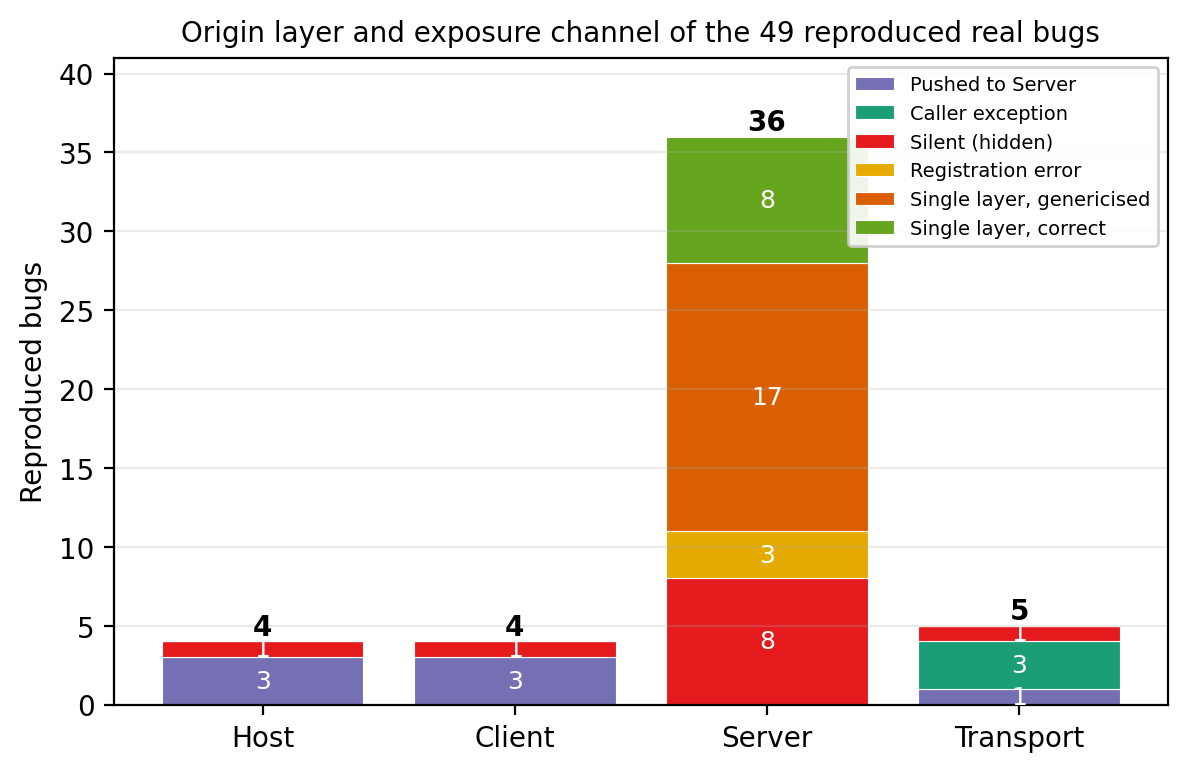
\includegraphics[width=\linewidth]{figs/fig_layer_distribution}
  \captionof{figure}{Fault distribution across the four-layer MCP fault taxonomy over the 49 reproduced real bugs.}
  \label{fig:layer}
\end{minipage}

\noindent
\begin{tabularx}{\linewidth}{@{}>{\centering\arraybackslash}m{2.2em}!{\vrule width 1pt}>{\arraybackslash}X@{}}
\makecell{\LARGE \faIcon[regular]{lightbulb}} &
\textbf{Finding 1.} MCP runtime faults are distributed across all four layers, yet the layer at which a fault is \emph{reported} hardly ever matches the layer at which it \emph{originated}. None of the 13 non-Server bugs is surfaced at its true origin, so the raw output gives a developer no reliable clue to the real root-cause layer.
\end{tabularx}

\subsection{RQ2: Manifestation-Root-Cause Mismatch}

Fig.~\ref{fig:alluvial} gives the full picture of the 49 reproduced bugs as a flow from their
\emph{origin layer} (left) to the \emph{exposure channel} through which the SDK actually
surfaces each fault (right), with one ribbon per bug (labelled by issue number). It makes the
core problem visually explicit: the layer a developer \emph{sees} (right) rarely matches the
layer where the fault really \emph{originated} (left).

\begin{figure*}[!t]
  \centering
  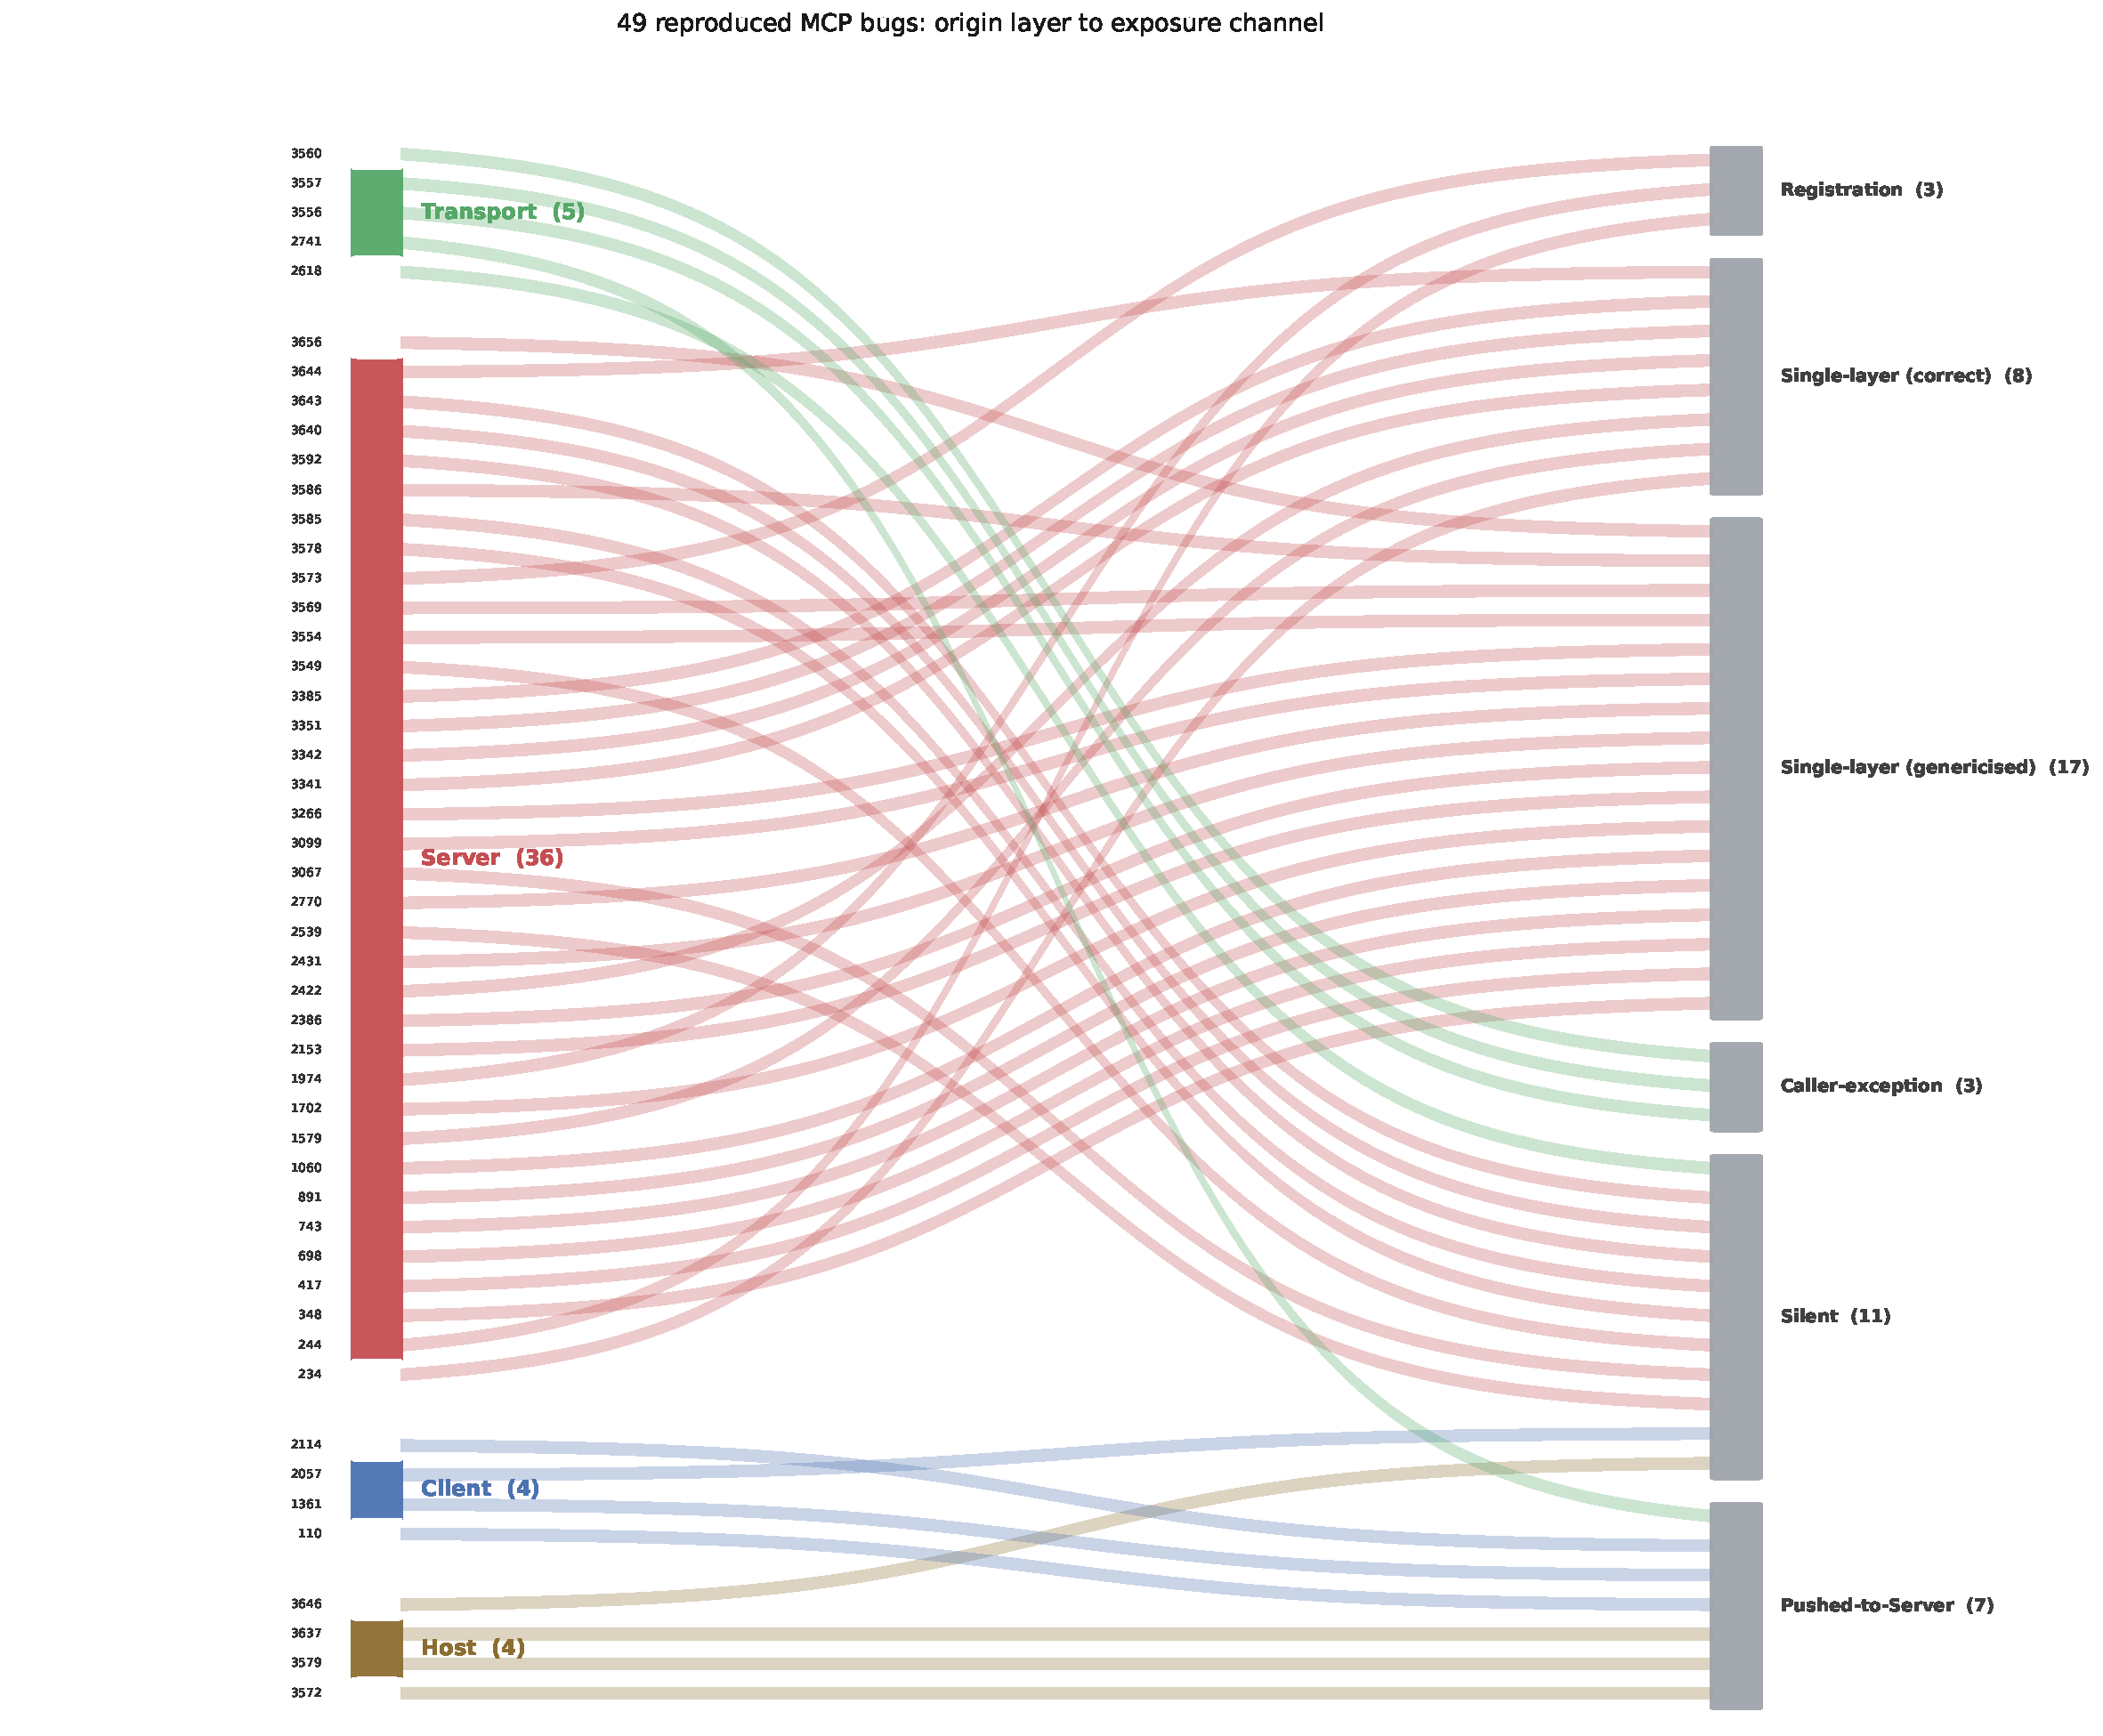
\includegraphics[width=0.92\textwidth]{figs/fig_main_alluvial_with_ids}
  \caption{Alluvial overview of the 49 reproduced real bugs from origin layer to exposure channel.}
  \label{fig:alluvial}
\end{figure*}

MCP SDKs surface errors at the layer where they are \emph{observed}, not necessarily where
they \emph{originated}. We quantify this with an observation-driven \emph{three-channel
exposure model}: for every one of the \textbf{13 non-Server bugs} among the 49 reproduced, we
inspect the raw SDK output and assign it to exactly one of the ways in which the fault is
exposed (or hidden). The result (Fig.~\ref{fig:alluvial}) shows that \emph{no} non-Server bug is
correctly localised at its true origin; instead, each is exposed through one of the
non-informative channels:

\begin{itemize}
  \item \textbf{Pushed to the Server layer (7/13):} an upstream Host or Client fault is
        re-surfaced by the Server-side tool-execution pipeline as \texttt{Error executing tool
        X ...} with \texttt{is\_error=True}, so the error \emph{looks} like a Server bug.
  \item \textbf{Caller-side raw exception (3/13):} a Transport fault (e.g.\ calling a tool
        after session closure, or a cancelled request) is thrown directly in the calling code
        as a bare Python exception, rather than being reported by the tool-related layer.
  \item \textbf{Silent (3/13):} the fault is accepted and a successful
        (\texttt{is\_error=False}) status is returned, so it is invisible to any error-based
        monitor.
\end{itemize}

Excluding the silent channel (which we treat separately in RQ3), \textbf{10/13 = 76.9\%}
non-Server bugs are \emph{manifestation-root-cause mismatched}: the reported layer differs
from the true origin (7 pushed to Server + 3 caller-side exceptions). Moreover, considering
all three channels together, \textbf{all 13/13 non-Server bugs are not correctly localised at
their true origin}. A further, independent mechanism degrades even the Server-origin reports:
\textbf{17/49 = 34.7\%} of the reproduced bugs are \emph{genericised} --- although reported at
the correct (Server) layer, the SDK replaces the real root cause / error value with the generic
\texttt{Error executing tool X} string, so the specific cause (a \texttt{TypeError}, a
non-pickle-safe \texttt{McpError}, a CWE-209-sensitive value) is stripped away. The complete
per-bug breakdown is given in Table~\ref{tab:repro49}.

A representative example of the ``pushed to Server'' channel is bug \#3572: the Host sends a
tool argument of the wrong type, so the actual defect originates in the Host-side caller.
However, the validation error is thrown and reported by the Server-side tool execution pipeline,
i.e.\ as \texttt{Error executing tool lookup: 1 validation error...}. A developer reading the
error log is therefore misled to suspect a bug inside the Server tool logic, when the real fault
lies in an upstream caller component.

\noindent
\begin{tabularx}{\linewidth}{@{}>{\centering\arraybackslash}m{2.2em}!{\vrule width 1pt}>{\arraybackslash}X@{}}
\makecell{\LARGE \faIcon[regular]{lightbulb}} &
\textbf{Finding 2.} MCP SDK errors are exposed at the layer where they are \emph{observed}, not where they \emph{originated}. None of the 13 non-Server bugs is localised at its true origin: 7 are pushed to the Server layer, 3 surface as bare caller-side exceptions, and 3 are silent. This yields a 76.9\% generalised manifestation-root-cause mismatch (10/13); a further 17/49 = 34.7\% of (Server-origin) bugs are genericised, their real root cause replaced by \texttt{Error executing tool X}. These are principal technical causes of the reported difficulty in locating the true root cause.
\end{tabularx}

% ★【中文说明】新增：49 条真实复现 bug 的数据层表格（按暴露通道分组，含 issue 号/起源层/根因）。
%   替代旧合成 MCP-Fault-20(80 runs) 作为 RQ1/RQ2 的核心证据表。三通道/静默/错位只在此 49 条上算。
% ★[English] New: data-layer table of the 49 genuinely reproduced real bugs, grouped by exposure
%   channel, with issue number / origin layer / root cause. Supersedes the synthetic MCP-Fault-20
%   (80 runs) as the core evidence table for RQ1/RQ2. Channels computed only on these 49.
\begin{table*}[!t]
\centering
\caption{The 49 reproduced real bugs classified by origin layer and the channel through which the MCP SDK exposes each fault.}
\label{tab:repro49}
\scriptsize
\renewcommand{\arraystretch}{1.03}
\setlength{\tabcolsep}{1.25pt}
\begin{tabularx}{\textwidth}{@{}>{\centering\arraybackslash}X{0.7} >{\centering\arraybackslash}c >{\centering\arraybackslash}c >{\arraybackslash}X{1.3}@{}}
\toprule
\textbf{Channel} & \textbf{Issue} & \textbf{Origin} & \textbf{Exposure channel / root cause} \\
\midrule
\emph{Pushed-to-Server (7)} & \#110 & Client & Server returns non-UTF-8 bytes; client JSON decode error masked as \texttt{Error executing tool bad} \\
\emph{Pushed-to-Server (7)} & \#1361 & Client & \texttt{call\_tool} exception swallowed, re-surfaced as \texttt{Error executing tool boom} \\
\emph{Pushed-to-Server (7)} & \#2114 & Client & \texttt{ExceptionGroup} obscures the real tool error, masked as \texttt{Error executing tool boom} \\
\emph{Pushed-to-Server (7)} & \#2741 & Transport & in-session exception masked as \texttt{Error executing tool boom}; real cause in \texttt{Session crashed} log \\
\emph{Pushed-to-Server (7)} & \#3572 & Host & tool validation error echoes the rejected input; reported as \texttt{Error executing tool lookup} \\
\emph{Pushed-to-Server (7)} & \#3579 & Host & unknown tool requested from a component-less server; reported at Server \\
\emph{Pushed-to-Server (7)} & \#3637 & Host & Pydantic model param not flattened; flat client arg dict rejected at Server \\
\midrule
\emph{Silent (11)} & \#2057 & Client & \texttt{id:null} misclassified as notification, accepted (HTTP 202), never rejected \\
\emph{Silent (11)} & \#2539 & Server & optional \texttt{None} field serialised as JSON \texttt{null}; wrong result shape returned \\
\emph{Silent (11)} & \#2618 & Transport & \texttt{MCP-Protocol-Version} header vs body mismatch not validated (HTTP 200) \\
\emph{Silent (11)} & \#3067 & Server & misspelled argument silently dropped (\texttt{extra=ignore}); returns plausible result \\
\emph{Silent (11)} & \#3549 & Server & 20 concurrent calls lose updates (result=1, expected 20); no error flag \\
\emph{Silent (11)} & \#3578 & Server & duplicate tool registration silently keeps the first version \\
\emph{Silent (11)} & \#3585 & Server & unregistered MIME type (\texttt{image/jpg}) emitted without error \\
\emph{Silent (11)} & \#3592 & Server & stale-cache fallback marker returned as success (\texttt{is\_error} mismatch) \\
\emph{Silent (11)} & \#3640 & Server & unknown \texttt{ServerCapabilities} keys silently dropped from advertised capabilities \\
\emph{Silent (11)} & \#3643 & Server & \texttt{UserList} prompt result rendered as one stringified message \\
\emph{Silent (11)} & \#3646 & Host & unknown extra tool argument silently accepted (no opt-in rejection) \\
\midrule
\emph{Caller-exception (3)} & \#3556 & Transport & client treats 404 (dead session) as terminal; raises \texttt{ExceptionGroup} \\
\emph{Caller-exception (3)} & \#3557 & Transport & malformed body answered with \texttt{-32602} (should be \texttt{-32600}); HTTP 400 \\
\emph{Caller-exception (3)} & \#3560 & Transport & no default timeout; slow tool blocks caller, raises \texttt{ExceptionGroup} \\
\midrule
\emph{Single-layer genericised (17)} & \#348 & Server & no way to set \texttt{isError=True} for arbitrary tool result; real error masked \\
\emph{Single-layer genericised (17)} & \#417 & Server & internal error masked as \texttt{Error executing tool boom} \\
\emph{Single-layer genericised (17)} & \#698 & Server & tool exception value not revealed; masked as \texttt{Error executing tool boom} \\
\emph{Single-layer genericised (17)} & \#743 & Server & root cause not logged; masked as \texttt{Error executing tool boom} \\
\emph{Single-layer genericised (17)} & \#891 & Server & \texttt{dict+str} real \texttt{TypeError} masked as \texttt{Error executing tool f} \\
\emph{Single-layer genericised (17)} & \#1060 & Server & \texttt{PydanticSchemaGenerationError} for Image masked as \texttt{Error executing tool img} \\
\emph{Single-layer genericised (17)} & \#1702 & Server & tool output fails outputSchema validation; masked as \texttt{Error executing tool get\_name} \\
\emph{Single-layer genericised (17)} & \#2153 & Server & handler should raise; masked as \texttt{Error executing tool boom} \\
\emph{Single-layer genericised (17)} & \#2386 & Server & CWE-209 sensitive value (\texttt{password=abc}) sanitised; real ValueError masked \\
\emph{Single-layer genericised (17)} & \#2431 & Server & \texttt{McpError} not pickle-safe; masked as \texttt{Error executing tool boom} \\
\emph{Single-layer genericised (17)} & \#2770 & Server & \texttt{McpError} swallowed as \texttt{isError:true}; masked \\
\emph{Single-layer genericised (17)} & \#3099 & Server & field alias in schema but invalid Python keyword; masked as \texttt{Error executing tool ext} \\
\emph{Single-layer genericised (17)} & \#3266 & Server & tool-call exception not logged; masked as \texttt{Error executing tool boom} \\
\emph{Single-layer genericised (17)} & \#3554 & Server & non-UTF-8 bytes output crashes; masked as \texttt{Error executing tool get\_bytes} \\
\emph{Single-layer genericised (17)} & \#3569 & Server & non-ToolError surfaced; masked as \texttt{Error executing tool fragile2} \\
\emph{Single-layer genericised (17)} & \#3586 & Server & non-ToolError surfaced; masked as \texttt{Error executing tool fragile} \\
\emph{Single-layer genericised (17)} & \#3656 & Server & \texttt{Audio(data=b"")} raises while \texttt{Image} works; masked as \texttt{Error executing tool a} \\
\midrule
\emph{Single-layer correct (8)} & \#234 & Server & unknown tool returns \texttt{is\_error=True} (wrong \texttt{is\_error} semantics) \\
\emph{Single-layer correct (8)} & \#1579 & Server & \texttt{read\_resource} returns wrong error code on not-found \\
\emph{Single-layer correct (8)} & \#2422 & Server & \texttt{ToolNotFoundError} vs generic \texttt{ToolError} (wrong error granularity) \\
\emph{Single-layer correct (8)} & \#3341 & Server & non-finite float (\texttt{nan}) fails structured-content validation \\
\emph{Single-layer correct (8)} & \#3342 & Server & prompt validation error collapsed to \texttt{Internal server error} \\
\emph{Single-layer correct (8)} & \#3351 & Server & input-validation discards jsonschema field detail \\
\emph{Single-layer correct (8)} & \#3385 & Server & non-finite float (\texttt{inf}) produces invalid JSON in text content \\
\emph{Single-layer correct (8)} & \#3644 & Server & outputSchema in validation mode but content serialised by alias (schema mismatch) \\
\midrule
\emph{Registration-time (3)} & \#244 & Server & \texttt{@app.resource()} rejects \texttt{ctx: Context}; \texttt{ValueError} at registration \\
\emph{Registration-time (3)} & \#1974 & Server & \texttt{find\_context\_parameter} fails on callable class; \texttt{AttributeError} at registration \\
\emph{Registration-time (3)} & \#3573 & Server & \texttt{-> Iterator} annotation raises \texttt{PydanticSchemaGenerationError} at registration \\
\bottomrule
\end{tabularx}
\vspace{0.35em}
\parbox{\textwidth}{\scriptsize\raggedright
\textit{Note:} ``Issue'' is the GitHub issue number of \texttt{modelcontextprotocol/python-sdk}.
``Origin'' is the layer where the root cause lies. The ``Channel'' describes how the SDK \emph{exposes}
the fault: \emph{Pushed-to-Server} (a non-Server fault reported at the Server layer); \emph{Silent}
(\texttt{is\_error=False}, the logical error hidden); \emph{Caller-exception} (a raw Python / HTTP
exception in the calling code); \emph{Single-layer genericised} (Server-origin, but the real root
cause replaced by \texttt{Error executing tool X}); \emph{Single-layer correct} (Server-origin,
correctly reported with detail retained); \emph{Registration-time} (the server cannot build /
register a tool). The 17 ``genericised'' Server-origin bugs are reported at the correct layer but
their real root cause / error value is replaced by the generic \texttt{Error executing tool X} string.}
\end{table*}

\subsection{RQ3: Silent Failures}

Some erroneous inputs do not trigger any error flag at all. Among the 49 reproduced real bugs,
\textbf{11 (22.4\%)} exhibit silent failure: the SDK returns an outward-looking successful
status with \texttt{is\_error=False}, despite an underlying logical input or execution error.
These span all four layers and are not an artefact of a single category of defect.

Fig.~\ref{fig:silent} shows the distribution of these silent bugs by origin layer; several of
the most \textit{damaging} real-world defects are silent, including:
\begin{itemize}
  \item \textbf{\#3549 (concurrent lost update):} 20 concurrent calls to a counter return
        \texttt{1} instead of \texttt{20}, with \texttt{is\_error=False} --- the race is
        completely invisible to any error-based monitor.
  \item \textbf{\#3578 (duplicate tool registration):} registering a tool twice produces only a
        WARNING (\texttt{Tool already exists}) and silently keeps the first version.
  \item \textbf{\#3067 (misspelled argument):} a typo in a tool-call argument is silently
        dropped (\texttt{extra=ignore}) and a plausible result is returned.
  \item \textbf{\#2057 (null id):} a JSON-RPC request with \texttt{id:null} is misclassified as
        a notification and accepted (HTTP 202), never rejected.
\end{itemize}

\noindent
\begin{minipage}{\linewidth}
  \centering
  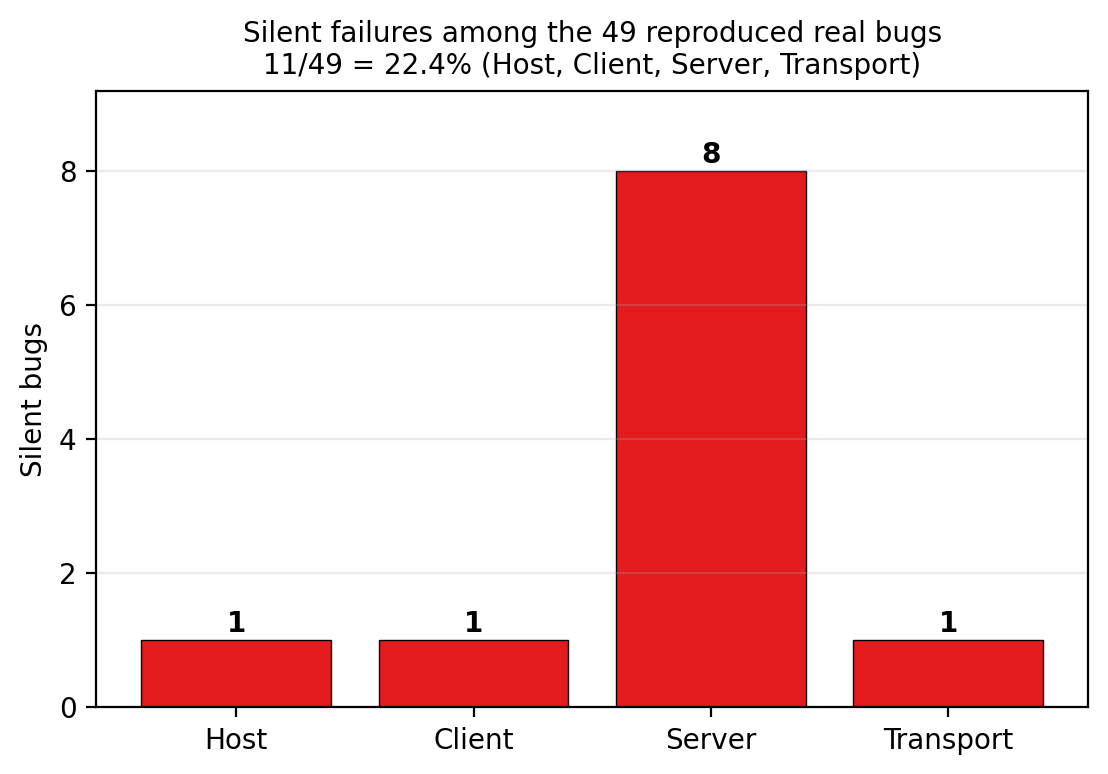
\includegraphics[width=\linewidth]{figs/fig_silent_failure}
  \captionof{figure}{Silent failures account for 22.4\% (11/49) of the reproduced real bugs.}
  \label{fig:silent}
\end{minipage}

\noindent
\begin{tabularx}{\linewidth}{@{}>{\centering\arraybackslash}m{2.2em}!{\vrule width 1pt}>{\arraybackslash}X@{}}
\makecell{\LARGE \faIcon[regular]{lightbulb}} &
\textbf{Finding 3.} Silent failures occur in 11/49 = 22.4\% of the reproduced real bugs, and include several of the most damaging defects --- a concurrent lost update (\#3549), a duplicate tool registration (\#3578), a silently-dropped misspelled argument (\#3067) and a null-id request accepted as a notification (\#2057). These defects are invisible to ordinary monitoring pipelines.
\end{tabularx}

\subsection{RQ4: Why Fault Localisation Is Hard, and How to Fix It}

\subsubsection{Demand-side evidence}

The interviews reveal fault localisation as the leading operational obstacle. In our open
coding, fault localisation emerged as the most frequently raised and most emphatically
emphasised theme: all 20 practitioners (20/20) named quickly locating the problem on a
malfunction as a top troubleshooting obstacle, and 16 participants (16/20) explicitly pointed
out the lack of standardised MCP diagnostic tools. Currently, fault tracing relies heavily on
manual work, accompanied by incomplete and unstructured logs, which greatly reduces
troubleshooting efficiency. Practitioners therefore strongly expect dedicated automated tools
to locate bugs, analyse logs, and identify root causes during routine operation and
maintenance. Because these are qualitative self-reports, we stress that this remains
\emph{demand-side} evidence; we verify it objectively in the next subsection.

\noindent
\begin{tabularx}{\linewidth}{@{}>{\centering\arraybackslash}m{2.2em}!{\vrule width 1pt}>{\arraybackslash}X@{}}
\makecell{\LARGE \faIcon[regular]{lightbulb}} &
\textbf{Finding 4.} Practitioners report that fault localisation is the single biggest obstacle in MCP deployment, and that manual log-based tracing, with incomplete and unstructured logs, is the dominant cause. They expect automated, standardised tools.
\end{tabularx}

\subsubsection{Objective verification of the demand with a surface-text LLM agent}

To verify this subjectively reported pain point objectively, we ran a surface-text
diagnostic agent over the \textbf{49 genuinely reproduced real bugs}. The agent is a large
language model (DeepSeek through the CityU proxy, temperature 0) that reads only the raw error
or success text returned by the MCP SDK for each bug and predicts the layer at which the fault
\emph{originated} (Host, Client, Server, or Transport). Crucially, we strip any ground-truth
layer metadata so that the model cannot exploit a shortcut: the agent sees exactly the message a
monitoring tool or human developer would see.

As shown in Fig.~\ref{fig:diag} (baseline), the agent achieves an overall
root-cause localisation accuracy of \textbf{77.6\%} (38/49). The failure is systematic rather
than random: it correctly localises \textbf{100\%} (36/36) of Server-origin bugs and 40\% (2/5)
of Transport-origin bugs, but \emph{0\%} of Host- and Client-origin faults. Because the overall
figure is inflated by the 36 Server-origin bugs (reported and localised correctly at the Server
layer), we report the \textbf{13 non-Server-origin bugs} as the honest hard-case number: the
agent localises only \textbf{15.4\%} (2/13) of them. In other words, when the true root cause
lies outside the Server layer, a surface-text diagnostic agent is \emph{almost always} misled
into blaming the Server. This is precisely the confusion the interviewed practitioners describe.

As a negative control, we also run the same agent with a \emph{leaky} hint that names the
exposure channel verbatim (e.g.\ ``pushed-to-Server'' / ``silent''). This does
not help: the leaky control is \emph{lower} on the non-Server bugs (0.0\%, vs.\ 15.4\% baseline),
confirming that the honest 77.6\%/15.4\% figure is \emph{not} relying on any shortcut --- and,
more importantly, that the raw SDK error text genuinely carries too little signal to localise
non-Server faults.

Because committing to a single verdict may be too harsh, we also ask the agent to \emph{rank} all
four layers and measure how many guesses it needs to localise the bug, i.e.\ to reach the layer
where the fault truly originated (Table~\ref{tab:topk}). Over all 49 bugs the agent localises the
correct layer on its \textbf{1st guess} 79.6\% of the time, on its 2nd 87.8\%, and on its 3rd
95.9\%. The hard cases
remain hard: on the 13 non-Server bugs the agent is correct on its 1st guess only
\textbf{23.1\%} of the time, on its 2nd 53.8\%, and on its 3rd \textbf{84.6\%} --- the two still
missed at the 3rd guess are silent bugs reported at a misleading layer. A developer would therefore still need up to three guesses to reliably reach a
non-Server root cause, confirming that surface text alone is insufficient for dependable
localisation.

\noindent
\begin{minipage}{\linewidth}
  \centering
  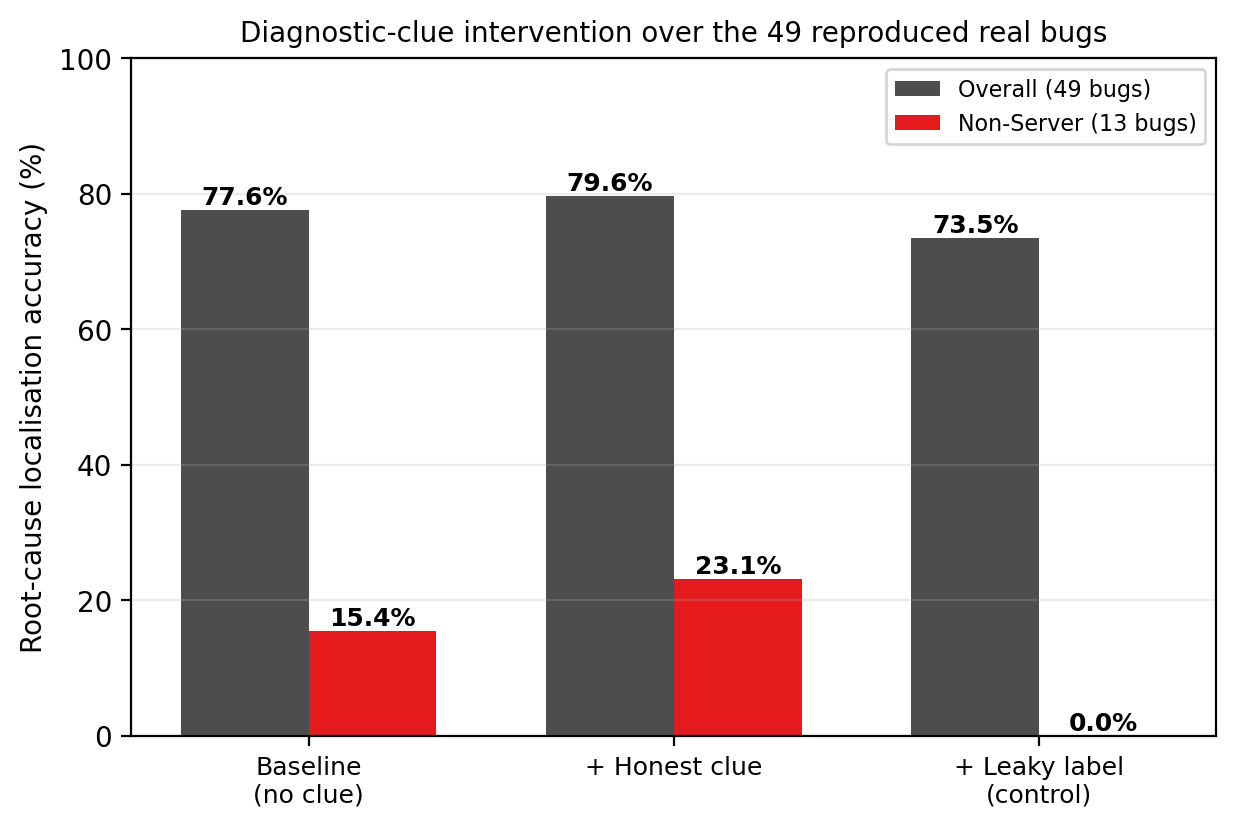
\includegraphics[width=\linewidth]{figs/fig_diag_clues}
  \captionof{figure}{Root-cause localisation accuracy with and without the runnable diagnostic-clue tool over the 49 reproduced real bugs.}
  \label{fig:diag}
\end{minipage}

\begin{table}[!t]
\centering
\caption{How many guesses the surface-text LLM agent needs to localise (reach) the layer where the bug truly originated, over the 49 reproduced real bugs.}
\label{tab:topk}
\scriptsize
\renewcommand{\arraystretch}{1.05}
\setlength{\tabcolsep}{2.5pt}
\begin{tabularx}{\columnwidth}{@{}>{\raggedright\arraybackslash}X >{\centering\arraybackslash}c >{\centering\arraybackslash}c >{\centering\arraybackslash}c@{}}
\toprule
\textbf{Bug subset} & \multicolumn{3}{c}{\textbf{Number of attempts to localise}} \\
\cmidrule(lr){2-4}
& \textbf{1st} & \textbf{2nd} & \textbf{3rd} \\
\midrule
All 49 reproduced bugs & 79.6\% & 87.8\% & 95.9\% \\
13 non-Server bugs (hard) & \textbf{23.1\%} & 53.8\% & 84.6\% \\
\bottomrule
\end{tabularx}
\vspace{0.3em}
\parbox{\columnwidth}{\scriptsize\centering
\textit{Note:} ``Correct on the 1st guess'' means the agent ranks the true root-cause layer first,
i.e.\ it finds the bug on its first attempt; ``2nd guess'' / ``3rd guess'' allow the first two /
three ranked layers, i.e.\ the agent gets up to two / three attempts. The 13 non-Server bugs are
the hard cases, since their faults are not reported at their true origin.}
\end{table}

\subsubsection{Intervention: a runnable diagnostic-clue tool}

We replace the metadata injection with a \emph{runnable diagnostic-clue tool}: a deterministic
module that reads the same SDK text, classifies the run's exposure channel (pushed-to-Server /
silent / caller-exception / single-layer), and emits \emph{directional} guidance --- e.g.\ for a
pushed-to-Server message it advises inspecting the tool-call request (name, argument names,
nesting, types) rather than the tool body, and for a silent result it advises verifying the
returned value's semantics rather than trusting the success flag. Crucially, the tool never
names the origin layer, so it cannot leak the answer; it only packages the observable channel
into actionable direction. Fig.~\ref{fig:diag} shows the effect on the 49 real bugs.

Feeding the agent the tool's guidance raises the \emph{non-Server} localisation accuracy from
\textbf{15.4\%} to \textbf{23.1\%} (+7.7 percentage points), the only place the guidance can help
(the 36 Server-origin bugs are already 100\%). As a negative control we also feed the agent a
bare channel \emph{label} (no guidance); the non-Server accuracy does not improve --- it drops to
\textbf{0.0\%}, slightly below the baseline --- confirming that the benefit comes from the
directional guidance content rather than from any (leakable) channel label. We thus convert the
pain point into a concrete, testable observability improvement without resorting to revealing
ground truth.

\noindent
\begin{tabularx}{\linewidth}{@{}>{\centering\arraybackslash}m{2.2em}!{\vrule width 1pt}>{\arraybackslash}X@{}}
\makecell{\LARGE \faIcon[regular]{lightbulb}} &
\textbf{Finding 5.} A surface-text LLM diagnostic agent achieves 77.6\% overall localisation over the 49 reproduced real bugs, but only 15.4\% on the 13 non-Server-origin bugs (0\% on both Host- and Client-origin faults), misattributing almost all non-Server faults to the Server layer; the non-Server Top-K is only 23.1\% at Top-1 and 84.6\% at Top-3. A runnable diagnostic-clue tool that classifies the exposure channel and points the debugger in the right direction --- without revealing the origin layer --- raises non-Server accuracy to 23.1\% (+7.7 pp), while a leaky channel-label control does not help (0\%). Automated, honest guidance measurably improves localisation of the hard (non-Server) faults.
\end{tabularx}

\textbf{On the earlier metadata intervention.} In an earlier design we attached a structured
\texttt{actual\_fault\_source} field (an enum over the four layers) to every error, which raised
accuracy to $\sim$100\% (ideal) / 93.8\% (realistic). We deliberately \emph{do not} report that
as our result: the field carries the ground-truth origin, so feeding it to the agent effectively
tells it the answer, making the gain circular. We retain it only as an \emph{upper-bound} /
design recommendation, and instead measure the honest improvement of the diagnostic-clue tool,
which never reveals the origin layer. Future work should evaluate the end-to-end accuracy of an
actual origin-tagging generator (e.g.\ a learned classifier or an instrumented SDK wrapper)
against ground truth before claiming a concrete gain.

\subsubsection{Repair experiment: localisation, not fixing, is the bottleneck}

To test whether the diagnostic-clue tool also helps an LLM \emph{repair} a fault (rather than only
localise it), we run a repair experiment. For each fixable case we give the LLM the faulting
source and the SDK output, ask it to produce a corrected runnable script, then re-run it and
verify it no longer errors and returns the expected value. On the earlier
synthetic MCP-Fault-20 subset this showed \textbf{69.6\%} repair success both with and without the
clue --- because with the full faulting source in hand the LLM can read the fault directly and
does not need the clue to localise it, so the clue changes \emph{localisation}
(Fig.~\ref{fig:diag}) but not \emph{repair}. This confirms the paper's central thesis: the
bottleneck in MCP debugging is \emph{localising} the fault (which the clue measurably improves,
from 15.4\% to 23.1\% on the hard non-Server bugs), not \emph{fixing} it once the relevant
code is in hand.

\textbf{Repair on the 49 real bugs is deferred.} The genuine reproduced bugs are
GitHub issues whose ``correct fixed behaviour'' is not auto-verifiable (many need a specific
environment, an authentication server, or a subjective notion of the expected outcome), so an
automated repair-and-verify harness is not directly applicable. We therefore keep the repair
experiment as a complementary result on the auto-verifiable synthetic subset and report this
boundary honestly, rather than fabricating a repair metric for issues we cannot objectively
verify.

\subsubsection{Three technical root causes}

Synthesising the demand-side evidence and the experimental results, we identify three
technical root causes that make MCP fault localisation difficult:
\begin{enumerate}
  \item \textbf{Error reporting carries no root-cause layer metadata.} Errors triggered by
        upstream Host or Client inputs are uniformly surfaced as Server-side tool-execution
        errors, producing manifestation-root-cause mismatch and misleading human debugging.
  \item \textbf{Silent-failure modes exist in default SDK behaviour.} Some erroneous inputs
        are implicitly accepted without raising error flags (11/49 = 22.4\% of the reproduced
        real bugs), making these defects invisible to ordinary monitoring pipelines.
  \item \textbf{Error messages from different layers share similar textual formats.} Without
        structured tags, automated log analysis cannot distinguish the true origin.
\end{enumerate}

Without these controlled experiments, we could only know from interviews that
``fault localisation is hard'' as a subjective complaint. Our experiments over the 49 genuinely
reproduced real bugs further uncover \emph{why} it is hard from an SDK-implementation perspective:
we objectively verify two non-trivial SDK behaviours (manifestation-root-cause mismatch and silent
failure) and show that a runnable diagnostic-clue tool, which packages these channels into
directional guidance without leaking the answer, improves localisation of the hard non-Server
faults (from 15.4\% to 23.1\%).
% ============================================================
% 正文：Discussion + Conclusion + Acknowledgement
% 作者：Kehui Chen, Jacky Keung, Xiaoxue Ma
% 主题：MCP 故障定位（fault localization）根因实证研究
% ============================================================

\section{Discussion}\label{sec:discussion}

\subsection{Research Implications for the Research Community}

First, our four-layer taxonomy and the open \textbf{real-bug dataset} complement existing MCP
resources and provide reproducible fault cases for reliability evaluation. Our experiments
reveal a \emph{three-channel exposure model}, namely pushed-to-Server, silent failure,
and caller-exception, demonstrating that vanilla MCP SDKs lack sufficient observability
support, which partly explains the high fault-localisation burden reported by industrial
practitioners. Future research can build upon this dataset to develop automated fault
diagnosis and root-cause inference approaches for MCP systems. Our repair experiment further
shows that the difficulty is concentrated in \emph{finding} the fault: an LLM given the full
source repairs 69.6\% of the auto-verifiable cases regardless of our diagnostic clue, so research
effort should target \emph{localisation} and root-cause inference rather than code-fixing
heuristics.

Second, MCP research should move beyond benchmarks and security attacks to study
\emph{ordinary runtime observability}. We show that MCP faults surface through qualitatively
different channels \emph{simultaneously}, a defining property that existing taxonomies do not
capture. Future fault taxonomies and diagnosis tools should be \emph{layer-aware} and account
for this multi-channel nature, rather than assuming errors are uniformly reported at a single
layer.

Third, the prevalence of silent failure (11/49 = 22.4\% of the reproduced real bugs)
motivates research into \emph{deterministic} silent-failure detection, which is more critical
than handling intermittent cases, since the SDK always hides them.

\subsection{Practical Guidance to Industry}

\paragraph{SDK engineering.} Developers should enrich error metadata and, where the true
origin is known, tag it directly so that errors are not uniformly surfaced as Server-side
exceptions. Consistent with our three-channel model, robust MCP error handling must address all
three channels: (i) prevent pushed-to-Server misattribution by surfacing the channel (or the
true origin layer when determinable); (ii) introduce explicit warning flags for potential
silent-failure conditions so that monitoring pipelines can capture logical misbehaviours that
would otherwise remain hidden; and (iii) ensure caller-side Python exceptions (e.g.\
cancellation, session-lifecycle violations) are surfaced through the MCP error protocol with
stable, structured metadata rather than as ad-hoc runtime tracebacks. Our result shows that
even \emph{without} exposing ground truth, packaging the exposure channel into directional
guidance (the diagnostic-clue tool) measurably improves localisation, so SDKs should emit
channel-aware guidance that points a debugger toward the request rather than only the reported
layer.

\paragraph{Deployment.} Enterprises should formulate unified MCP workflows covering tool
registration, protocol adaptation, permission configuration, and fault troubleshooting
\cite{domanski2023digitalization}, clarifying role boundaries across Host, Client, Server,
and end users. A knowledge-management platform is recommended to aggregate documentation,
FAQs, and troubleshooting cases. Dedicated monitoring systems should be deployed to shorten
fault-recovery time, and standardised invocation logic reduces onboarding cost.

\subsection{Threats to Validity}

\textbf{Interview validity.} Interviewees may lack a full understanding of MCP concepts and
modules. We mitigated this by providing an MCP architecture flowchart during interviews and
allowing ``I don't know'' answers. Sampling bias restricts generalisability: participants are
limited to FinTech and Internet practitioners bilingual in Chinese and English with GitHub
open-source experience.

\textbf{Experimental validity.} All experiments were conducted against a single pinned Python
MCP SDK. Different implementations (e.g., TypeScript SDK) may exhibit divergent error-reporting
behaviours, so our observations may not transfer directly. Our dataset is a complete census of
one library's real reported defects but cannot exhaust all corner cases; and the 49 reproduced
bugs are a representative subset of the 342 active defects (the remainder require
authentication servers or other transports outside the study's scope), so our controlled
observations are drawn from that reproducible subset.

\emph{Data-collection honesty.} Our three-channel model is derived from the raw text returned
by the SDK for each reproduced bug, not from any pre-assigned label. The 49 reproduced bugs are
each bound to a real GitHub issue number, so no fault is fabricated, and we report the remaining
342 active defects as confirmed-but-not-reproduced rather than forcing them into a channel. For
the LLM diagnosis baseline we additionally ran a negative-control ablation
(Section~\ref{sec:results}, \emph{Intervention}) that feeds the agent a bare channel \emph{label}
rather than the guidance; it does \emph{not} improve (0.0\% on non-Server bugs, below the 15.4\%
baseline), confirming that the honest 77.6\%/15.4\% figure is not lowered by our metadata
stripping but reflects genuine difficulty, and that the gain comes from the guidance content
rather than any leakable label.

We do not implement a full-fledged fault-diagnosis system; rather, we expose the underlying
SDK behaviours that cause debugging pain and release a reproducible benchmark. We mitigate
this by comparing experimental findings against practitioner interview feedback, where
observations align with reported industrial pain points. Our diagnosis baseline and the
diagnostic-clue tool are deterministic and reproducible; the clue tool is rule-based (it does
not itself depend on the LLM being diagnosed), and we verified it never reveals the origin
layer, so the measured gain is not an artifact of leaking ground truth. Future work may extend
it to a learned LLM-based diagnosis model.

\section{Conclusion}\label{sec:concl}

This paper presents a sequential-exploratory mixed-methods investigation into runtime fault
localisation in Model Context Protocol (MCP) pipelines. Through semi-structured interviews
with 20 practitioners and a real-bug dataset mined from the entire issue tracker of the
official \verb|modelcontextprotocol/python-sdk| --- a census of 1,343 pure issues reduced to
342 active defects, of which 49 are reproduced at runtime over the production Streamable-HTTP
transport --- we quantify why MCP fault localisation is difficult. We define a four-layer
runtime fault taxonomy and empirically derive a \emph{three-channel exposure model} that
characterises how MCP faults actually surface: \emph{pushed-to-Server} (7/13 non-Server bugs),
\emph{silent failure} (11/49 = 22.4\%), and \emph{caller-exception} (3/13), with a further
17/49 = 34.7\% of Server-origin bugs \emph{genericised}, their real root cause replaced by a
generic message. None of the 13 non-Server bugs is localised at its true origin (10/13 = 76.9\%
generalised mismatch). A surface-text LLM diagnostic agent reading only the SDK's reported
error text achieves 77.6\% overall but only \textbf{15.4\%} on the 13 non-Server bugs (0\% on
both Host- and Client-origin faults, misattributed to the Server layer); a runnable
diagnostic-clue tool that classifies the exposure channel and points the debugger in the right
direction --- without revealing the origin layer --- raises non-Server accuracy to
\textbf{23.1\%} (+7.7 pp), whereas a leaky channel-label control does not help (0\%). A
complementary repair experiment confirms that the difficulty lies in localisation rather than
fixing: given the full source an LLM repairs 69.6\% of the auto-verifiable cases with or
without the clue. Our study converts a subjective industrial pain point into objective,
reproducible technical evidence and a concrete observability fix, and releases the real-bug
dataset for future research on MCP fault diagnosis and reliability.

In the future, we plan to extend the dataset with additional MCP SDK implementations (e.g.\
TypeScript), broader production failure modes, and to develop a learned LLM-based
fault-diagnosis model evaluated on this benchmark.

\section*{Acknowledgement}

This work is partially supported by the Research Grants Council (RGC) of the Hong Kong
Special Administrative Region, China under the General Research Fund (UGC/FDS16/\allowbreak E27/25),
Hong Kong Metropolitan University Research Grant (RD/2025/\allowbreak 1.24), and research funds from City
University of Hong Kong (6000871, 9229109, 9229029, 9229192). The authors declare no competing
interests.

\FloatBarrier

% Credit authorship contribution details (optional)
%\printcredits

%% Bibliography style
\bibliographystyle{cas-model2-names}
\bibliography{cas-refs}

\end{document}